\sectionlang{sv}{Experimentellt genomförande}
\sectionlang{en}{Experimental procedure}
\label{sec:exper}
\lang{sv}{
För att kunna analysera reaktionshastigheten behöver ni kunna följa
reaktionens gång som funktion av tid. Till ert förfogande kommer ni att ha en
s.k. ``stopped-flow''-utrustning (se \cref{fig:stopped-flow-schematic,fig:stopped-flow-photo}).
}
\lang{en}{
  In order to analyze the rate of reaction, you will need to follow the reaction duing time.
  To your aid you will have a ``stopped-flow''-apparatus (see \cref{fig:stopped-flow-schematic,fig:stopped-flow-photo}).
}
% TODO: subfloat:
\begin{figure}[h]
  \centering
  \subfloat[][Schematisk representation]{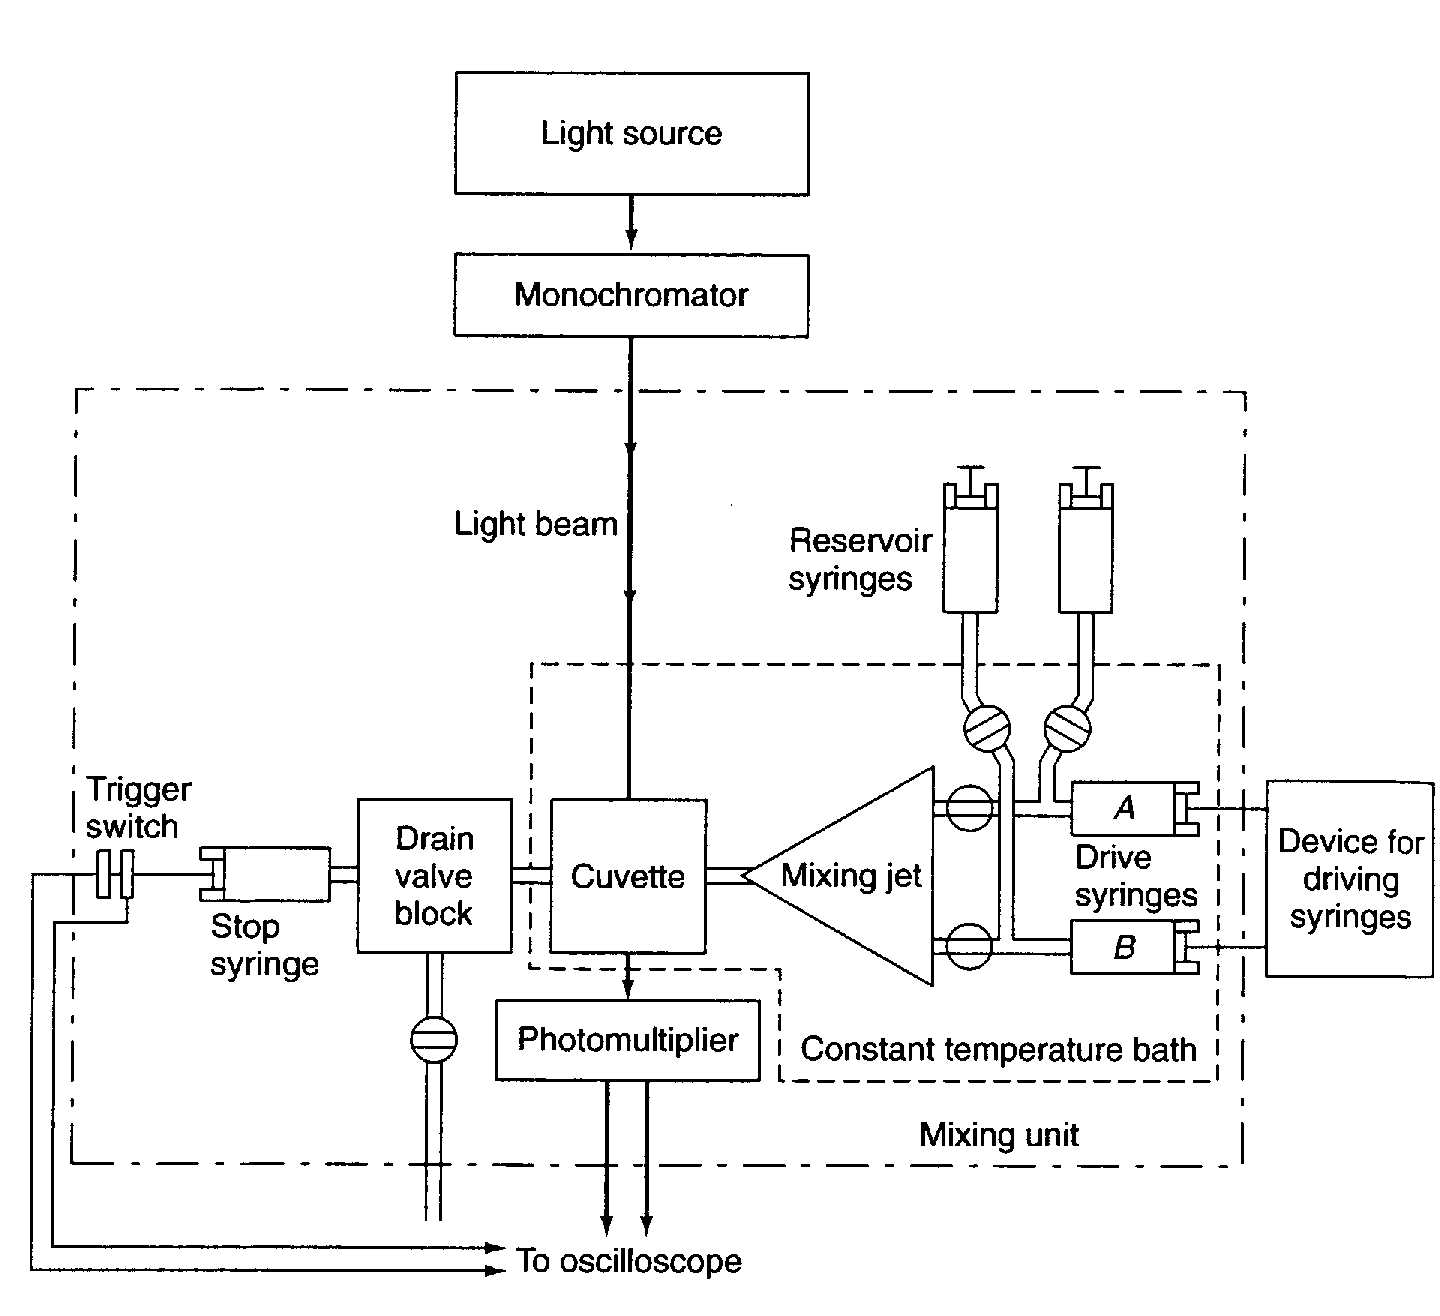
\includegraphics[scale=0.15]{fig/stopped_flow.png} \label{fig:stopped-flow-schematic}}
  \subfloat[][Foto av uppställning]{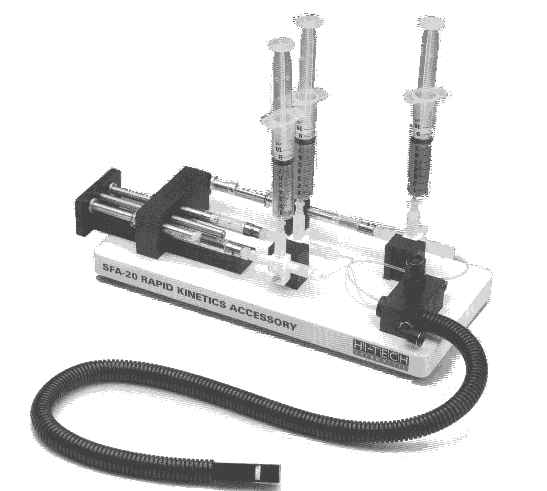
\includegraphics[scale=0.2]{fig/setup_bw3.jpg} \label{fig:stopped-flow-photo}}
  \caption{Stopped-flow utrustning}
\end{figure}

\lang{sv}{
Blandkammaren är termostaterad med hjälp av vattenbad som ni själva får
välja temperatur för. Ni kan börja era försök vid
rumstemperatur, temperaturintervallet ni kan arbeta inom styrs av
temperaturen av kallvattnet i husets ledningar (säg \SI{15}{\celsius})
och hastigheten för reaktionen. 

Kyvettens längd är \SI{1}{\centi\metre} (vilket
tillsammans med extinktionskoefficienten  är något ni har nytta av att
veta när ni väljer koncentrationsintervall för era reaktantlösningar).

Ni kommer att använda er utav en dator med ett interface
skrivet i LabView. Handhavandet av programmet är beskrivet i
\cref{sec:handhavande}. Från varje försök kommer ni att erhålla dataserier med
absorbans som funktion av tid vid en våglängd som ni själva väljer. Dessa
tidsserier kommer sparas i form av textfiler som ni sparar på USB minne
som ni själva tar med er till laborationstillfället.
}
\lang{en}{
  The mixing chamber is under temperature control through the use of a water
  bath for which you must choose a temperature. You will begin your experiments at room temperature,
  the temperature window in which you may work is determined by the temperature of the cold water
  in the tap and (say \SI{15}{\celsius})
  and the rate of the reaction. 

The cuvette is \SI{1}{\centi\metre} long (which
together with the extinctioncoefficient allows you to choose concentrations for your
solutions).

You will use a computer with an interface written in LabView. The usage of the program is described
in \cref{sec:handhavande}. From each run you will obtain data series with 
absorbance \emph{vs.} time at a wavelength of your choice. These
time sereis will be saved as text files on a USB memory stick that you yourselves need to bring to the 
lab.
}
\subsectionlang{sv}{Stamlösningar}
\subsectionlang{en}{Stock solutions}
\lang{sv}{
För att bereda era två reaktantlösningar kommer ni att ha tillgång till följande
stamlösningar:
}
\lang{en}{
  To prepare your two reactant solutions you will need access to the following stock solutions:
}

\begin{itemize}
\item \SI{2}{\Molar} \ce{NaClO4}
\item \SI{2}{\Molar} \ce{HClO4}
\item \SI{100}{\milli\Molar} \ce{KSCN}
\item \SI{100}{\milli\Molar} \ce{Fe(ClO4)3} + \SI{200}{\milli\Molar} \ce{HClO4}
\end{itemize}

\lang{sv}{
Eftersom blandkammaren inte är perfekt är det viktigt att båda
reaktantlösningarna får samma jonstyrka och pH.
}
\lang{en}{
Since the mixing chamber is imperfect it is important that both reactant solutions have the same ionic strength and pH.
}
\subsectionlang{sv}{Handhavande}
\subsectionlang{en}{Usage}
\label{sec:handhavande}
\lang{sv}{
Nedan finner ni en instruktion för handhavandet av
laborationsutrustningen och programvaran. Enheten för tidsangivelserna är
millisekunder i programmet.
}
\lang{en}{
  Below you will find an instruction for the usage of the apparatus and software.
  The unit for time is milliseconds.
  }

\begin{figure}[h]
  \centering
  \subfloat[][Intensitets-vy]{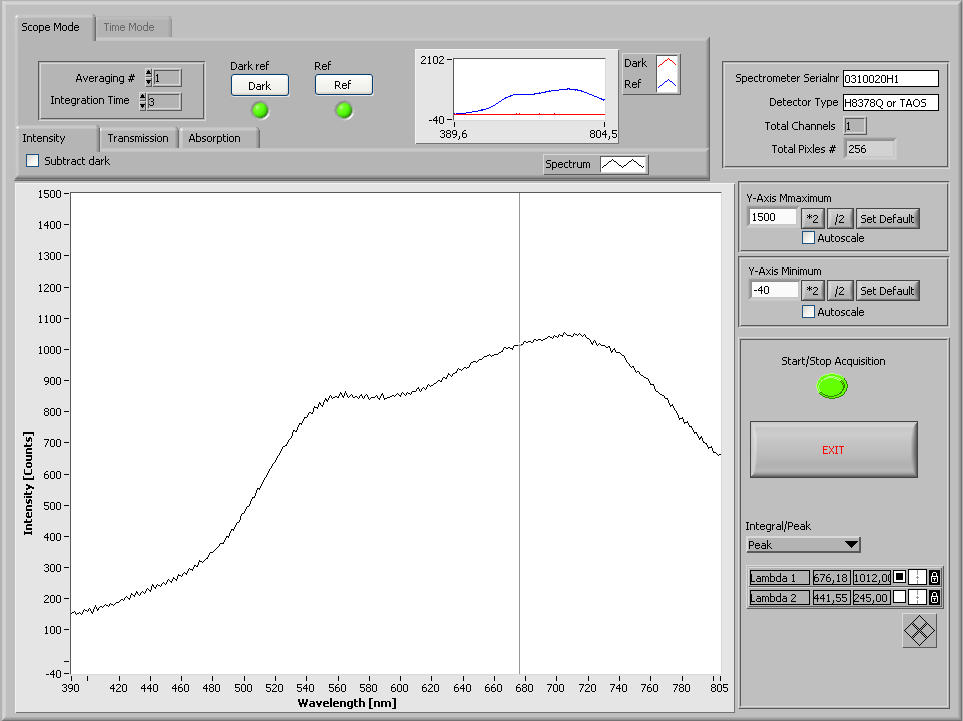
\includegraphics[scale=0.13]{fig/intensity.png}  \label{fig:intensity}}
  \subfloat[][Transmissions-vy]{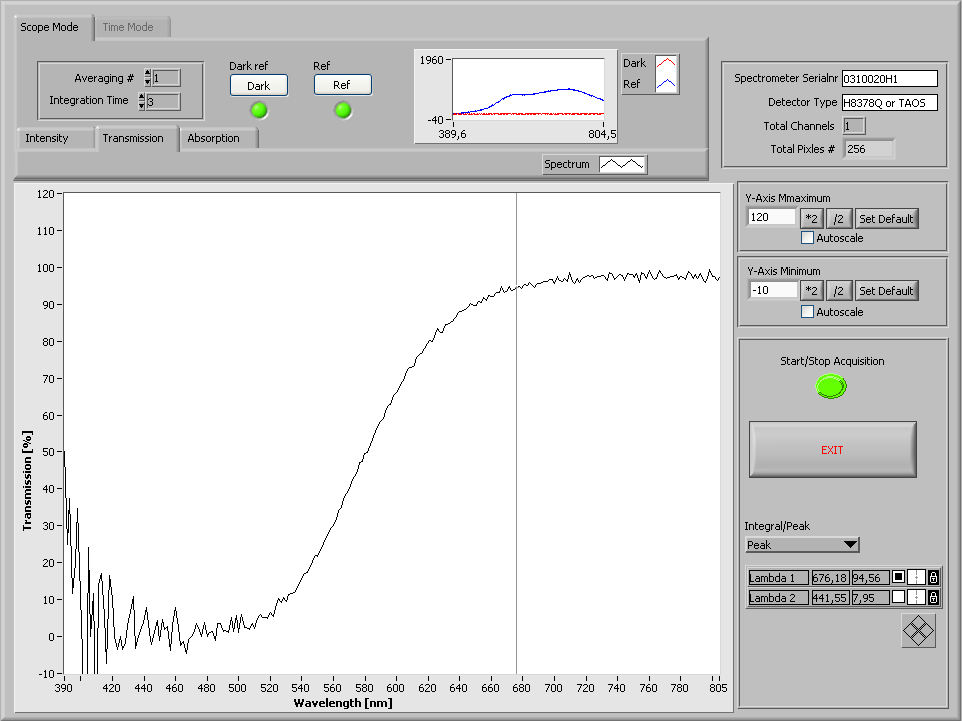
\includegraphics[scale=0.13]{fig/transmission.png} \label{fig:transmission}}
  \subfloat[][Absorptions-vy]{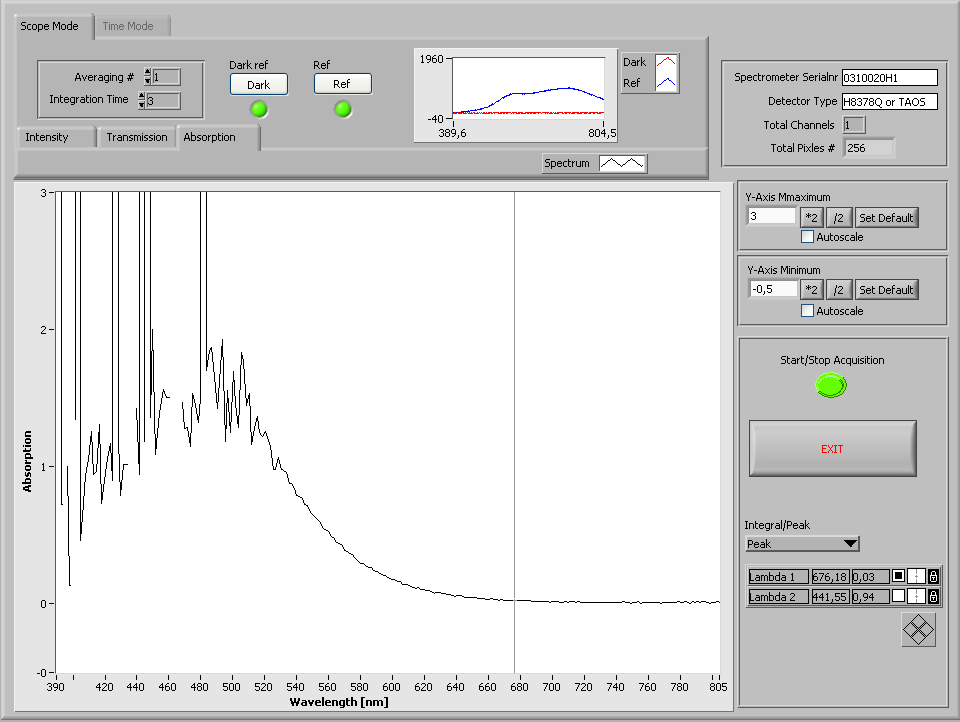
\includegraphics[scale=0.13]{fig/absorption.png} \label{fig:absorption}}
  \caption{LabView baserat interface för datainsamling.}
\end{figure}


\subsubsectionlang{sv}{Förberedelser}
\subsubsectionlang{en}{Preparations}
\lang{sv}{
\begin{itemize}
\item Tänd spektrofotometerns lampa minst 5 minuter innan mätningarna.
\item Kontrollera att vattennivån är inom de markerade gränserna för vattenbadet.
Starta termostat, välj temperatur och lägg i extern termometer.
\item Kontrollera att termostaterat vatten flödar genom uppställningen
  med hjälp av den röda flödesmätaren.
\item Sätt på kranvattnet.
\item Starta programmet ``StopFlowSpect'' på datorn.
\item OBS! Vid alla mätningar och
  kalibreringar ska knappen för ``Start/Stop Acquisition`` vara röd. Om
  programmet stängs av måste kalibreringen (med dest. vatten) göras om,
  tryck därför aldrig på ``Exit''.
\item Undvik att luftbubblor kommer in i kyvetten.
\end{itemize}

\subsubsection{Kalibrering}
\begin{itemize}
\item Ställ ``Integration time'' till 2 ms.
\item Blockera strålgången med metallplåten. Tryck på ``Dark'' (en röd
  plan linje med brus bör visas). Ta bort
  metallplåten.
\item Injicera destillerat vatten. Tryck på ``Ref'' (en blå linje
  motsvarande lampans spektrum bör visas). (se \cref{fig:intensity})
\item Kontrollera att transmittansen och absorptionen ser ut som de
  bör (100\% transmittans, 0 absorbance) (Tryck ``Start/Stop acquisition'').
\item Byt sprutor och injicera reaktantlösning tills komplex bildats i
  utloppet. (se \cref{fig:transmission,fig:absorption})
\item Se till att ``Start/Stop acquisition'' är deaktiverad (röd). Gå in i
  absorptionsfönstret och välj våglängd för mätningarna genom att välja
  ``Peak'' i Integral/peak-menyn och ``drag-drop'':a den vertikala
  linjen. Beakta att det viktiga måttet vid val av våglängd är
  förhållandet mellan signal och brus (``signal-to-noise-ratio''), denna
  uppskattar ni genom att aktivera ``Start/stop acquisition''.
\end{itemize}

\subsubsection{Mätning}
\begin{itemize}
\item Gå in på fliken ``Time mode''.
\item Välj ``As fast as possible'', ``Save to file'' och ``Use a trigger''.
\item Tryck på ``Start'' så att den gröna lampan intill ``Running'' lyser
  (datorn väntar nu på att brytaren vid stoppet för produktsprutans kolv aktiveras).
\item Vinkla samtliga T-kranar nedåt.
\item Injicera snabbt in ny reaktantlösning. Håll kvar greppet i 4 sekunder.
\item Välj alltid ``Replace'' ifall överskrivning efterfrågas (kopiera
  och döp om {\tt data.txt} om ni är nöjda, genväg finns på skrivbordet, eller {\tt
    C:\textbackslash temp\textbackslash data\textbackslash
    data.txt}). Upprepa mätningen ett flertal gånger (säg 5) och spara
  undan filerna (t.ex. {\tt 1.txt, 2.txt, ..., 5.txt}). Ni kommer
  genomföra en statistisk analys på dessa replikat.
\end{itemize}
}
\lang{en}{
\begin{itemize}
\item Turn on the spectrophotometer lamp at least 5 minutes before the measurements.
\item Check that the water level is within the selected water bath limits.
Start thermostat, select temperature and load in external thermometer.
\item Check that thermostated water flows through the installation
  Using the red flowmeter.
\item Turn on tap water.
\item Start the program `` StopFlowSpect '' on your computer.
\item NOTE! At all measurements and
  Calibrations, the `` Start / Stop Acquisition`` button should be red. If
  If the program is turned off, the calibration (with the destination water) must be done again,
  Never press `` Exit ''.
\item Avoid air bubbles coming into the cuvette.
\end{itemize}

\subsubsection{Calibration}
\begin{itemize}
\item Set `` Integration time '' to 2 ms.
\item Block the beam path with the metal plate. Press `` Dark '' (one red
  Plan line of noise should be displayed). Remove
  Metal sheet.
\item Inject distilled water. Press `` Ref '' (a blue line
  The corresponding lamp's spectrum should be displayed). (See \ cref {fig: intensity})
\item Check that the transmittance and absorption look like them
  Should (100 \% transmittance, 0 absorbance) (Press `` Start / Stop acquisition '').
\item Replace syringes and inject reactant solution until complexes are formed
  Outlet. (See \ cref {fig: transmission, fig: absorption})
\item Make sure `` Start / Stop acquisition '' is deactivated (red). Walk into
  Absorption window and select the wavelength of the measurements by selecting
  `` Peak '' in the Integral / peak menu and `` drag-drop '': a the vertical
  The line. Note that the important measure when selecting wavelength is
  The signal-to-noise ratio ratio, this
  You appreciate activating `` Start / stop acquisition ''.
\end{itemize}

\subsubsection{Measurement}
\begin{itemize}
\item Enter the `` Time Mode '' tab.
\item Select `` As fast as possible '', `` Save to file '' and `` Use a trigger ''.
\item Press `` Start '' so that the green light next to `` Running '' lights up
  (The computer is now waiting for the switch at the stop for the product spray piston to be activated).
\item Angle all T-cranes downwards.
\item Quickly inject new reactant solution. Hold the grip for 4 seconds.
\item Always select `` Replace '' if overwriting is requested (copy
  And rename {\ tt data.txt} if you are satisfied, shortcut exists on the desktop, or {\ tt
    C: \ textbackslash temp \ textbackslash data \ textbackslash
    Data.txt}). Repeat the measurement several times (say 5) and save
  Remove the files (eg {\ tt 1.txt, 2.txt, ..., 5.txt}). You come
  Perform a statistical analysis on these replicates.
\end{itemize}
}
%%% Local Variables:
%%% mode: latex
%%% TeX-master: "../main"
%%% ispell-local-dictionary: "swedish"
%%% End:
